\documentclass[main.tex]{subfiles}
\begin{document}
\section{Introduction}

\subsection{Dead Reckoning}\label{sec:deadReckon}
% explain the issues of dead Reckoning
% use as an introduction: 
% 	to the FWKin prob.
% 	to the different sensors used

%todo: fix 1st sent.

Robot localization is crucial to effective robot locomotion. Various methods are
used to determine the current and future locations of robot; each unique to the
available sensors, robot structure and environment. Dead reckoning is one of the
simpler methods used. It requires as few sensors as possible and relies mostly
on known motion models and states.  Dead reckoning is a method of finding the
location of an object based on a known motion model and current state
information. Once the current state of an object is known then its motion model
can be used to predict future motion states. For example, one can predict the
future position of a robot if it is known that that the robot is moving in a
straight line and at a constant speed and its current position.

A two wheeled robot as shown in \figref{2wheelBot} will be used for our analysis
of dead reckoning. Two wheeled odometry is used to create a motion model of the
robot which is then used to predict future locations of the robot. In this study
only the $x$ and $y$ coordinates are of interest although velocity can easily
derived. 

\begin{figure}[H]
\begin{center}
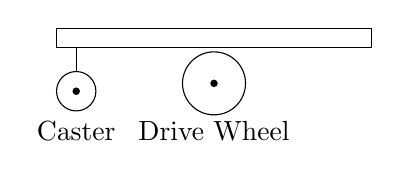
\begin{tikzpicture}
	\begin{scope}[shift={(.25,0)}]
		\node at (0,-.5) {Caster};
		\draw (0,.55) -- (0,0);
		\draw [fill=white](0,0) circle[radius=.25];
		\draw[fill=black] (0,0) circle[radius=.04];
	\end{scope}

	\draw (0,.55) rectangle (4,.8);

	\begin{scope}[shift={(2,0)}]
		\node at (0,-.5) {Drive Wheel};
		\draw (0,.10) circle[radius=.4];
		\draw[fill=black] (0,.10) circle[radius=.04];
	\end{scope}
\end{tikzpicture}

\end{center}
\caption{2 Wheeled Robot (Side view)}
\label{fig:2wheelBot}
\end{figure}

We will begin our analysis with the odometry model of the two wheeled robot. The
odometry model is as follows (its derivation is beyond the scope of this
report):

\begin{equation}
\label{eq:deadReckonState}
	P(t) = 
	\begin{bmatrix}
	S \\ \theta
	\end{bmatrix}
	=
	\begin{bmatrix}
	\frac{1}{2}	& \frac{1}{2} \\[0.3em]
	\frac{1}{\mathrm{w}} & -\frac{1}{\mathrm{w}}
	\end{bmatrix} 
	\begin{bmatrix}
	S_R(t) \\ S_L(t)
	\end{bmatrix}
\end{equation}

Where $S$ and $\theta$ respectively are the robot distance travelled and heading
of the robot. $S_L$ and $S_R$ are the distances traveled by each wheel (left and
right respectively). $w$ is the distance between the contact points of the
wheels of the robot.

\begin{figure}[H]
	\begin{center}
	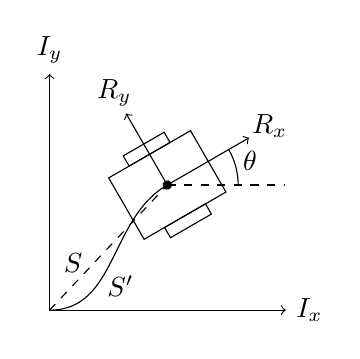
\begin{tikzpicture}[scale=3]
% axis labels
\node at (0,1.1) {$I_y$};
\node at (1.1,0) {$I_x$};

% inertial axis
\draw[<->] (0,1) -- (0,0) -- (1,0);

% robot reference frame
\begin{scope}[rotate around={30:(0.4,0.3)},shift={(0.4,0.3)}]
%wheels 
	\draw (.1,0) rectangle (.3,-0.05);
	\draw (.1,.3) rectangle (.3,.35);
	%robot body
	\draw (0,0) rectangle (0.4,0.3);
	% axis
	\coordinate (C) at (.2,0.15);
	\draw[fill=black] (C) circle [radius=0.05em];
	\draw[<->] (.2,.5) -- (.2,0.15) -- (0.6,0.15);
	% rotation angle
	\begin{scope}[rotate around={-30:(.2,0.15)},shift={(.2,0.15)},dashed]
		\draw[dashed] (0,0) -- (.5,0);
		\draw[solid] (0.3,0) arc [start angle=0,end angle=30, radius=.3];
		\node at (.35,0.1) {$\theta$};
	\end{scope}
	% axis labels
	\node at (.2,.6) {$R_y$};
	\node at (.7,.15) {$R_x$};
\end{scope}
% robot position line
\node at (.1,.2) {$S$};
\draw[-,dashed] (0,0) -- (C);
% robot curve line
\draw (0,0) to [out=0,in=210] (C);
\node at (.3,.1) {$S\mathrm{'}$};
\end{tikzpicture}

	\end{center}
	\caption{Robot Motion Model from $t=0 -$ \delt}
	\label{fig:2wrMotion}
\end{figure}


From \eqref{deadReckonState} we can create a motion model relative to the
inertial frame of reference $I$ (as shown in \figref{2wrMotion}). To simplify
our analysis the following is assumed:

\begin{itemize}
\item The robot's motion model is measured on a time differential \delt that
is small with respect to the total time ($T$) the robot performs its motion. 
\item The robot's wheel encoders are error-less and no wheel slipping occurs.
\item \delt is chosen to be small enough so that $S\mathrm{'}-S \approx 0$ and
thus $S\mathrm{'} = S$.
\end{itemize}

From these assumptions we have a motion model for the robot:

\begin{equation}
\label{eq:motionState}
\xi_{i} = 
\begin{bmatrix}
x \\ y \\ \theta
\end{bmatrix}
=
\begin{bmatrix}
\cos{\theta} & 0\\
\sin{\theta} & 0\\
0 & 1
\end{bmatrix}
P(t_i+\Delta\mathrm{t})-P(t_i)
\end{equation}

$\xi_{i}$ is the position of the robot after some time lapse \delt. Thus to get
the current position of the robot after some time $T$ simply sum the interval
position changes\footnote{A continuous form of \eqref{sumE} is beyond ths scope
of this lab and is not needed computationally.}: 

\begin{equation}
\label{eq:sumE}
\xi(T) = \xi_0 + \sum^{n}_{i=0} \xi_{i} : n = \frac{T}{\Delta\mathrm{t}}
\end{equation}

\eqref{sumE} simply means that given the robots initial position ($\xi_0$) and a sequence
of wheel distance measurements for $t=\{\delT,2\delT,\cdots,T\}$ the position of
the robot at $T$ can be predicted. This of course is only valid for the above
assumptions.

%TODO: add section on inertial to robot frame of reference rotation matrix

Dead reckoning is not practical when used alone. Sensor noise, wheel slippage,
and distance estimation error ($S-S\mathrm{'}$) all affect the outcome of
\eqref{sumE}. However dead reckoning is not completely useless. In fact it forms
the base motion model for other filter and motion estimation algorithms (such as
the Kalman filter\footnote{\url{https://en.wikipedia.org/wiki/Kalman_filter}}).

\subsection{Wheel Encoders}
% encoding) measuring x/v/a from encoders sources of error

As seen in \eqref{deadReckonState} the robot's motion model is dependent on
wheel distance travelled. Sensors that can translate rotational wheel motion to
linear distance traveled are called wheel encoders. Different types of encoders
are available each with their advantages and disadvantages. In this study we
will examine a quadrature wheel encoder. 

A quadrature encoder uses a disk (as shown in \figref{quadEncode}) and two
optical sensors to track the position of a wheel. The disk is patterned with
alternating opaque and transparent wedges. As the disk spins the optical sensors
produce a logic signal (0 or 1) respective to the wedge type it is over. The two
sensors are placed in such a manner that their outputs are $90\degree$ out of
phase (see \figref{encSig}). The encoder is coupled with the wheel in such a
manner that the disk spins with an angular velocity that is proportional to that
of the wheel.

\begin{figure}[h]
	\begin{center}
	\usepgflibrary{shapes.geometric}
% optical sensor A
\tikzset{
	sensor/.pic={
		\node at (0,.3) {#1};
		\draw (-.2,0.1) rectangle (.2,.2);
		\draw (-.1,0.1) to [out=-90,in=-90] (.1,0.1);
	}
}
\tikzset{
	wedge/.pic={
	\draw[fill=#1] (0,0) -- (1,0) arc [start angle=0,end angle=45,radius=1] -- (0,0);
	}
}
% optical sensor B
\begin{tikzpicture}[scale=3]
%sensors
\draw (0,1) pic [rotate=0,scale=3] {sensor=A};
\draw (.924,.383) pic [rotate=-67.5,scale=3] {sensor=B};

\draw[fill=white] (0,0) circle[radius=1];
\draw[fill=black] (0,0) circle[radius=0.4em];

\foreach \ang in {0,90,...,270}
	\draw (0,0) pic[rotate=\ang,scale=3] {wedge=black};
\end{tikzpicture}

	\end{center}
	\caption{Quadrature Encoder}
	\label{fig:quadEncode}
\end{figure}

\begin{figure}[h]
	\begin{center}
	\tikzset{
	dsig/.pic={
	\node at (4.5,1) {#1};
	\draw (0,0) -- (1,0) -- (1,1) -- (2,1) -- (2,0) -- (3,0) -- (3,1) -- (4,1);
	}
}

\begin{tikzpicture}[scale=3]
\draw[<->] (0,1) -- (0,0) -- (2,0);
\draw pic[shift={(0,2)}] {dsig=A};
\draw (0,.2) -- (.15,.2) pic {dsig=B};
\end{tikzpicture}

	\end{center}
	\caption{Quadrature Encoder Signals ($90\degree$ phase shift)}
	\label{fig:encSig}
\end{figure}

\begin{table}[h]
	\begin{center}
	\begin{tabularx}{.35\textwidth}{ccc}
		\toprule
		Phase & A Signal & B signal\\
		\midrule
		0 & 0 & 0 \\
		1 & 1 & 0 \\
		2 & 1 & 1 \\
		3 & 0 & 1 \\
		\bottomrule
		\end{tabularx}
		\caption{Phases of Quadrature Encoder}
		\label{tab:phaseTab}
	\end{center}
\end{table}

The output from the encoder can be viewed as a 4 phase signal (see
\tabref{phaseTab}). Each phase change is called a ``pulse'' and is detected by
an observing hardware (typically a MCU). Software can then be used to determine
the rotation state of the wheel by analyzing the encoder phase after every pulse
it produces.

The direction of the encoder can be determined by two successive phase changes.
For example if the current phase is 2 and on the next encoder reading the phase
is now 1 the encoder is rotating clockwise. If determining the encoder phase is
not performed within a certain amount of time then the software will miss some
encoder ticks resulting in erroneous calculations. 

Because the encoder uses wedges to indicate rotation the encoder's resolution is
restricted to a certain number of pulses per rotation angle. This means that
their is a minimum distance the wheel must travel in order for the encoders to
detect motion.

The lateral distance that each wheel travels is: 

\begin{equation}
\label{eq:encTransDist}
S_{L,R} = R\mu\sum_{i=0}^n{(-1)^{f(\rho_i,\rho_{i-1})}}
\end{equation}

Where $S_{L,R}$ is the lateral distance of the wheel traveled, $\mu$ is the
encoder resolution in units of $[\frac{radians}{pulse}]$, $n$ is the number of
pulses, and $R$ is the radius of the wheel the encoder is coupled with.
$f(\rho_i,\rho_{i-1})$ is a function that takes the ``current'' phase and the
previous phase and returns $2$ or $1$ if the direction between the two phases
is forward or reverse respectively.

The
translational velocity of the wheels can be found from \eqref{encTransDist}:

\begin{equation}
\label{eq:encTransSpeed}
\dot{S}_{L,R} = \frac{S_{L,R}}{\delT}
\end{equation}

Note that \delt is the same as that defined in \secref{deadReckon}. This 
allows synchronization between the movement of the robot to the quantifying of
the robot motion state. 

\subsection{Sonar Range Finder}

\end{document}
